% Conclusions chapter text
\chapter{Conclusions and Future Research}
\label{Ch7}

\raggedbottom
\clearpage

One of the fundamental goals of Earth science is to understand, in a predictive manner, how the global carbon cycle adapts and responds to external perturbations, both in the past as well as the future. The importance of this knowledge becomes especially apparent in the context of anthropogenic climate change -- how will Earth's natural cycles respond to this massive unnatural forcing? As a conclusion, I propose a set of thought experiments to highlight how the results contained within this thesis might offer novel insight into this understanding, and bring attention to the work that lies ahead.

\section{Rivers in the global carbon cycle}

It has long been realized that atmospheric \ce{CO2} concentrations (\textit{p}\ce{CO2}) have remained relatively stable throughout much of Earth's history despite global-scale variability in tectonics, temperature, ice cover, etc. Therefore, to prevent runaway \ce{CO2} emission (\textit{i.e.} "hot-house" climate) or consumption (\textit{i.e.} "ice-house" climate), it is canonically thought that the global carbon cycle is controlled by an intricate network of positive and negative feedback mechanisms acting over geologic timescales (\SIrange{~ e6}{e7}{yr}). This interpretation inherently implies that \textit{p}\ce{CO2}, and therefore global temperature via the greenhouse effect, is the "master variable" to which all feedbacks respond \citep[Figure \ref{Ch7Fig:1}][]{Ebelman:1845uw,Berner:1999wj}.

Throughout the last half century, many feedbacks governed by fluvial processes have been proposed that involve a direct link between temperature and mechanisms acting to increase or decrease \textit{p}\ce{CO2}. One of the most widely invoked is the idea that the rate of \ce{CO2} drawdown due to silicate rock weathering followed by \ce{CaCO3} deposition in marine sediments is a function of global temperature, which, in turn, is a function of atmospheric \textit{p}\ce{CO2} \citep[\textit{e.g.}][]{Goldschmidt:1933tg,Rubey:1951ha,Walker:1981wn}. Increasing \textit{p}\ce{CO2} therefore increases silicate weathering rates, especially in mountainous regions \citep{Maher:2014kq}, leading to elevated \ce{CO2} drawdown until a stable equilibrium is once again reached. Acting in parallel is the erosion and efficient export of OC derived from the terrestrial biosphere (OC\sub{bio}), which is additionally biased toward high-elevation catchments \citep{FranceLanord:1997ua,Galy:2007ev,Hilton:2008fo,Galy:2015fx}. According to this mechanism, if increased \textit{p}\ce{CO2} leads to elevated erosion due to an acceleration of the hydrologic cycle, then OC\sub{bio} export and burial will subsequently increase, drawing down \textit{p}\ce{CO2}. Both of these mechanisms therefore emphasize the importance of elevation and catchment geometry in regulating feedback sensitivity.

% Figure 1
\begin{figure}[h]
	\makebox[\textwidth][c]{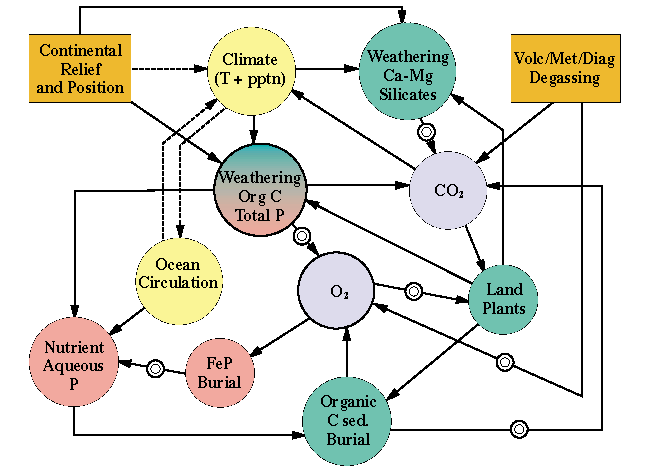
\includegraphics[]{Thesis_Figures/Ch7Fig1}}
	\caption[Carbon cycle feedback network \textit{a la} Berner]{Carbon cycle feedback network as described by Berner. Arrows with small concentric circles represent negative feedbacks, while arrows without circles represent positive feedbacks. Color scheme is as follows: blue, atmosphere; green, surficial carbon processes; pink, surficial phosphorus processes; yellow, other surficial processes; orange, tectonic processes. Figure modified from \citet{Berner:1999wj}.}
	\label{Ch7Fig:1}
\end{figure}

However, they are likely balanced by positive feedbacks acting to amplify \textit{p}\ce{CO2} perturbations. The two most significant pertaining to river catchments involve \ce{CO2} emissions due to the oxidation of rock-derived ("petrogenic") organic carbon \citep[OC\sub{petro};][Chapter \ref{Ch6}]{Hilton:2014dh} or the oxidation of pyrite followed by subsequent dissolution of \ce{CaCO3} \citep{Torres:2014cx}, both of which should accelerate under warmer conditions, especially in mountainous catchments \citep{Torres:2016bd}. While the controls on these mechanisms is just beginning to be understood, the importance of high-elevation regions with high sediment yield is already clear. Based on the this emerging understanding, I propose a nuanced update to this paradigm -- namely, that \ce{CO2} source and sink processes can directly respond to the same perturbation without invoking a feedback loop that includes temperature.

For example, OC\sub{petro} oxidation appears to be rapid and not kinetically limited, at least given the erosion rates observed in Taiwan, suggesting that increasing exposure of bedrock material to the surface via erosion will increase the rate of OC\sub{petro} oxidation (a \ce{CO2} source) in addition to OC\sub{bio} burial and silicate weathering (\ce{CO2} sinks). However, this relationship should break-down under extraordinarily high erosion rates, as bedrock incision would export significant amounts of unweathered OC\sub{petro} and relatively little OC\sub{bio}, dampening both mechanisms \citep{Hilton:2011jw}. One important future direction for the work presented in Chapter \ref{Ch6}, therefore, is to constrain microbially mediated OC\sub{petro} oxidation rates and fluxes in catchments experiencing a wide range of erosion rates and to determine the kinetic limits of this mechanism. Additionally, it is critical that we understand the relationship, if any, between OC\sub{petro} yield in fluvial sediments and oxidation fluxes on landscapes. Combined, this would allow us to predictively constrain \ce{CO2} emissions due to OC\sub{petro} oxidation a function of sediment yield, as has been done previously for OC\sub{bio} export \citep{Galy:2015fx}. Furthermore, the \ce{CO2} emission fluxes and governing mechanisms controlling pyrite weathering remain almost completely unknown \citep{Calmels:2007fk,Torres:2014cx}, presenting a pressing need for future research. 

Still, with regards to organic carbon, the framework proposed here suggests that the net effect of fluvial systems as an atmospheric \ce{CO2} source or sink and their sensitivity to \textit{p}\ce{CO2} perturbations is a function of erosion rate. To probe this conceptual understanding, first I consider a high-elevation Earth surface similar to that of Taiwan, while still allowing erosion rates to vary over many orders of magnitude. In this scenario, the fraction of OC\sub{petro} oxidized ($f_{\text{ox}}$) appears to be \SI{<15}{\%} of the total yield due to high rates of bedrock incision and rapid export of unweathered material \citep{Hilton:2011jw}. Using the power law relationships between OC\sub{bio}, OC\sub{petro}, and suspended sediment yield of \citet{Galy:2015fx}, and assuming that \SI{<15}{\%} of the OC\sub{petro} yield in rivers is oxidized to \ce{CO2}, fluvial OC processes in this conceptual Earth would represent a net \ce{CO2} sink until global sediment yield increased above \SIrange{~ e4}{e5}{t.km^{-2}.yr^{-1}}, depending on OC\sub{bio} burial efficiency (Figure \ref{Ch7Fig:2}, blue shaded region). The magnitude of rivers as a \ce{CO2} sink would be maximized at slightly lower yields, between \SI{e3}{t.km^{-2}.yr^{-1}} and \SI{e4}{t.km^{-2}.yr^{-1}}, and would decrease to zero with decreasing erosion.

% Figure 2
\begin{figure}[h]
	\makebox[\textwidth][c]{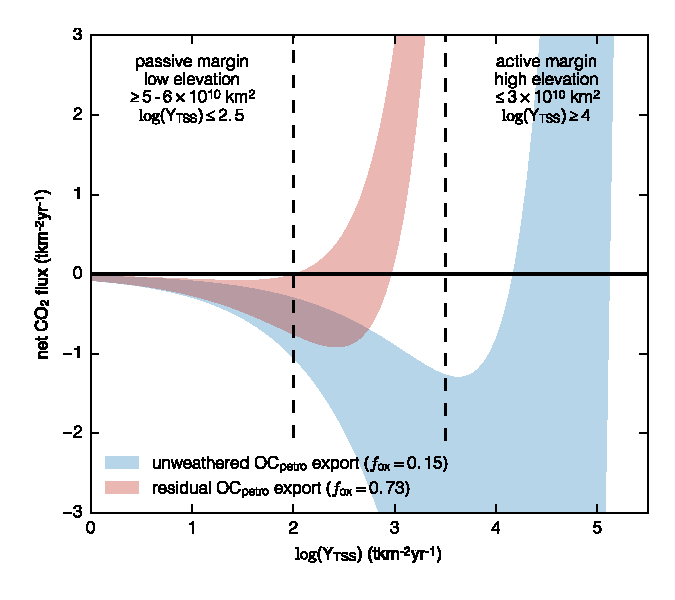
\includegraphics[]{Thesis_Figures/Ch7Fig2}}
	\caption[Riverine \ce{CO2} source/sink as a function of sediment yield]{Conceptual diagram showing the net effect of fluvial OC processes (\textit{i.e.} OC\sub{bio} burial, OC\sub{petro} oxidation) on atmospheric \ce{CO2} as a function of sediment yield. Two extreme fractional OC\sub{petro} oxidation values ($f_{\text{ox}}$) are considered. Shaded regions represent a range of OC\sub{bio} burial efficiencies from \SIrange{30}{100}{\%}. Yield relationships from \citet{Galy:2015fx}.}
	\label{Ch7Fig:2}
\end{figure}

At the opposite extreme, I consider a case where all fluvially exported OC\sub{petro} is the residual of oxidation on landscapes -- that is, uplift is fast enough to continuously expose fresh bedrock to the surface, but low enough to prevent landsliding and incision, therefore preventing the export of unweathered OC\sub{petro}. Assuming the $f_{\text{ox}}$ value of $73^{+2}_{-3}$ \% calculated in Chapter \ref{Ch6} applies globally, OC\sub{petro} oxidation in this scenario out-paces OC\sub{bio} burial above a sediment yield of \SIrange{~ e2}{e3}{t.km^{-2}.yr^{-1}} (Figure \ref{Ch7Fig:2}, red shaded region), similar to the modern global average of \SI{176}{t.km^{-2}.yr^{-1}} \citep{Galy:2015fx}. In reality, there likely exists a transition between the high-$f_{\text{ox}}$ scenario at low sediment yield and the low-$f_{\text{ox}}$ scenario at high sediment yield. Nonetheless, these thought experiments demonstrate the high sensitivity of counter-balancing positive and negative feedbacks in active margin systems that respond, in parallel, to the same \textit{p}\ce{CO2} perturbation. Understanding this relationship will form an important component of my future research.

Finally, I consider how a low-elevation Earth would respond to \textit{p}\ce{CO2} changes. For passive-margin, climate-controlled systems such as the Congo River, the results of Chapters \ref{Ch4} and \ref{Ch5} indicate that exported POC is largely derived from downstream regions, and that hydrology is a key control on OC source. Because both silicate weathering and OC\sub{bio} burial flux would decrease in this low-erosion system relative to modern Earth, fluvial feedbacks would become less efficient at regulating atmospheric \textit{p}\ce{CO2}. This can be seen by the fact that net \ce{CO2} flux due to OC processes is largely insensitive to changes in sediment yield in passive margins, regardless of $f_{\text{ox}}$ (Figure \ref{Ch7Fig:2}). While limited in geographic extent today, a low-elevation Earth could be described by significant proliferation of permanently inundated swamp-forest regions such as the middle Miocene Pebus System located in the modern-day Amazon basin \citep{Hoorn:1994vz}. Using the \textit{Cuvette Congolaise} as an example, this would likely lead to an increase in terrestrial OC storage and longer fluvial residence times due to widespread anoxia. Therefore, OC\sub{bio} storage in intermediate anoxic reservoirs could become more important in determining the role of rivers as a negative feedback to \textit{p}\ce{CO2} perturbations in this end-member system. 

The results of Chapter \ref{Ch5}, combined with those of \citet{Schefuss:2016cp}, suggest that the ability of anoxic reservoirs to act as an atmospheric \ce{CO2} sink depends on hydrology and discharge. When \textit{p}\ce{CO2} is high and the hydrologic cycle is amplified, high discharge through lowland depressions would expand the geographic extent of anoxic soils and therefore stabilize this OC reservoir \citep{Schefuss:2016cp}. However, as \textit{p}\ce{CO2} declines leading to lower monsoon intensity and lower discharge, these regions could become exposed and oxidized, not entirely unlike what is occurring in modern-day permafrost soils. Chapters \ref{Ch4} and \ref{Ch5} of this thesis highlight the importance of anoxic regions in driving OC export from large, passive-margin systems despite their small geographic extent \citep[\textit{e.g.} the \textit{Cuvette Congolaise} constitutes \SI{\approx 4}{\%} of the total Congo Basin;][]{Mayaux:2004uw}.

\section{A final thought}

In reality, Earth exists between these two extremes. While the end-members presented here provide a useful thought exercise, to properly understand fluvial responses to \textit{p}\ce{CO2} perturbations we must turn to systems such as the Amazon or Ganges-Brahmaputra that contain both high-erosion headwaters \textit{and} large floodplains. In the coming years, I plan further investigate the importance of OC\sub{petro} oxidation and OC\sub{bio} export, in addition to pyrite weathering, by incorporating time-series sample sets from such systems. Furthermore, I stress the importance of continuing the collaborations and time-series sample collection presented in this thesis. To fully constrain the response of fluvial carbon cycle to a changing climate, in addition to the threats currently posed by deforestation and land-use change, it is critical that we continue these analyses and generate multi-decadal records of riverine OC export.

Lastly, I emphasize the utility of developing novel instrumental methods. One of the main challenges facing organic geochemists is the fact that any given sample contains a complex OC mixture representing a rage of chemical composition, environmental residence time, and susceptibility to degradation. Only by continuing to push the technical envelope will we be able to sufficiently meet this challenge.

